\documentclass[12pt, twoside]{article}
\usepackage[letterpaper, margin=1in, headsep=0.2in]{geometry}
\setlength{\headheight}{0.6in}
%\usepackage[english]{babel}
\usepackage[utf8]{inputenc}
\usepackage{microtype}
\usepackage{amsmath}
\usepackage{amssymb}
%\usepackage{amsfonts}
\usepackage{siunitx} %units in math. eg 20\milli\meter
\usepackage{yhmath} % for arcs, overparenth command
\usepackage{tikz} %graphics
\usetikzlibrary{quotes, angles}
\usepackage{graphicx} %consider setting \graphicspath{{images/}}
\usepackage{parskip} %no paragraph indent
\usepackage{enumitem}
\usepackage{multicol}
\usepackage{venndiagram}

\usepackage{fancyhdr}
\pagestyle{fancy}
\fancyhf{}
\renewcommand{\headrulewidth}{0pt} % disable the underline of the header
\raggedbottom
\hfuzz=2mm %suppresses overfull box warnings

\usepackage{hyperref}

\fancyhead[LE]{\thepage}
\fancyhead[RO]{\thepage \\ Name: \hspace{4cm} \,\\}
\fancyhead[LO]{BECA / Dr. Huson / Geometry\\*  Unit 2: Angles\\* 4 October 2022}

\begin{document}

\subsubsection*{2.5 Extension: Convert between radians and degrees \hfill CCSS.HSG.SRT.C.8}

Use this graduated circle, marked in both radians and degrees, to convert angle measures.\\
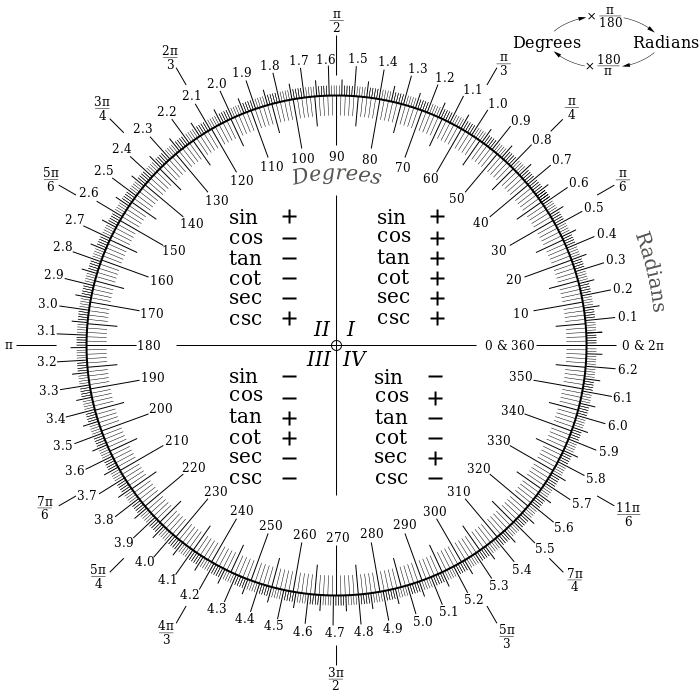
\includegraphics[width=16cm]{../graphics/Degree-Radian_Conversion.png}
\begin{enumerate}
\item Convert radians and degrees. (nearest whole degree, nearest hundredth radian).\vspace{.25cm}
  \begin{multicols}{2}
    \begin{enumerate}
      \item $40^\circ = $ \vspace{1cm}
      \item $65^\circ = $ \vspace{1cm}
      \item $150^\circ = $
      \item $\displaystyle 1.1 =$ \vspace{1cm}
      \item $\displaystyle 0.55 =$ \vspace{1cm}
      \item $\displaystyle 2.1 =$
    \end{enumerate}
  \end{multicols} \vspace{1cm}

\newpage
Express the result to the nearest hundredth. (Degree measures to whole degrees)
\begin{multicols}{2}
  \item $\displaystyle \tan 70^\circ = $ \vspace{1cm}
  \item $\displaystyle \tan 1.4 \,\rm{radians}= $ \vspace{1cm}
  \item $\displaystyle \tan^{-1} (\frac{6}{5}) = $ \hspace{2.4  cm} degrees \vspace{1cm}
  \item $\displaystyle \tan^{-1} (\frac{91}{250}) = $ \hspace{2cm} radians \vspace{1cm}
  \begin{flushright}
    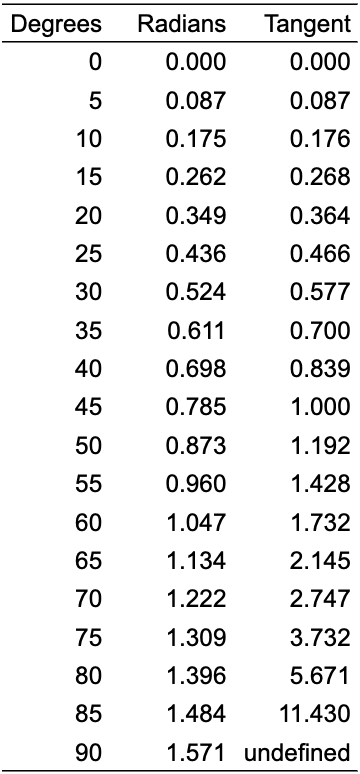
\includegraphics[width=6cm]{../graphics/Degree-radian-tangent-table.png}
  \end{flushright}
\end{multicols}

Challenge
\item Find the value, rounding to the nearest hundredth.\\[0.25cm]
$c=\sqrt{(-6.125)^2+(\sqrt{90.1})^2}$
\vspace{2cm}

\item Solve for $x$\\[0.25cm]
 $7=\sqrt{6x-11}$

\end{enumerate}
\end{document}
